\section{Existentialism is a Database Theory}
% Existentialism is a Humanism
% - Jean-Paul Sartre

\begin{marginfigure}
	\centering
	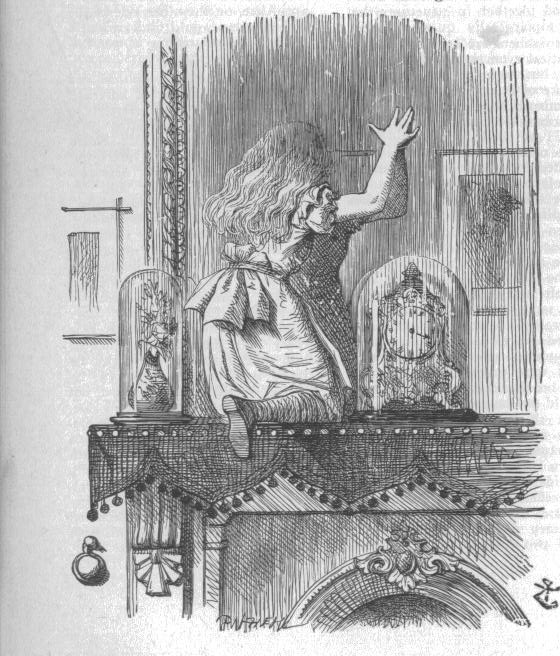
\includegraphics[width=\linewidth]{fig/intro/aliceroom.jpg}
	\caption{Looking glass room, by John Tenniel.}
\end{marginfigure}

We think of problems of the form $\textsf{query} \homto^? \textsf{data}$
as existential problems: for instance, if $\?G$ is the "graph@@dir" with
two nodes $u$ and $v$ and a single edge from $u$ to $v$,
then asking if there is a "homomorphism" from $\?G$ to a graph $\?H$ amounts
to asking if there exists at least one edge in $\?G$.

As we would expect for any existential problem, they are monotonic:
if a solution exists, and we add more data, then a solution still exists.
More formally, for any "structure" $\?A$, $\?B$ and $\?B'$, if $\?B$ is a "substructure"
of $\?B'$ and $\?A \homto \?B$,
then $\?A \homto \?B'$.

The example of SQL queries (\Cref{ex:sql-as-hom}) is actually more than a mere example:
every "homomorphism problem" $\?A \homto \?B$ can be seen as a SQL query evaluation problem
where $\?A$ encodes a "query@@sem" in the \textsf{SELECT-WHERE-FROM}
fragment of SQL and $\?B$ is a relational database.
This fragment can also be characterized as the fragment
of "first-order logic" where universal quantification, union and negation are not allowed.
For instance, the SQL query of \Cref{ex:sql-as-hom} can be expressed by the formula
\begin{align*}
	\phi(\textsf{title}, \textsf{time}) \defeq\; 
	& \exists \textsf{movie\_id}.\, 
	\exists \textsf{length}.\, 
	\exists \textsf{director}.\,
	\exists \textsf{room\_id}.\, \\
	& \hphantom{\land~} \textsc{Movies}(\textsf{movie\_id}, \textsf{title}, \textsf{length}, \textsf{director}) \\
	& \land
	\textsc{Projections}(\textsf{movie\_id}, \textsf{room\_id}, \textsf{time}).
\end{align*} 
\begin{marginfigure}
	\centering
	\begin{tikzpicture}
		\node (a0) at (-.1,5.2) {};
		\node (a1) at (-.4,3.5) {};
		\node (a2) at (-.1,1.8) {};
		\node (a3) at (.1,1.8) {};
		\node (a4) at (.4,3.5) {};
		\node (a5) at (.1,5.2) {};

		\node (b0) at (-.2,5.2) {};
		\node (b1) at (-.8,3.1) {};
		\node (b2) at (-.5,1.5) {};
		\node (b3) at (-.4,.6) {};
		\node (b4) at (-.2,-.2) {};
		\node (b5) at (.2,-.2) {};
		\node (b6) at (.4,1) {};
		\node (b7) at (.2,1.4) {};
		\node (b8) at (-.5,2.6) {};
		\node (b9) at (-.4,3.8) {};
		\node (b10) at (.2,5.2) {};
	
		\draw[use Hobby shortcut, closed=true, draw=c2, fill=c2, fill opacity=.4] 
			(b0) .. (b1) .. (b2) .. (b3) .. (b4) .. (b5) .. (b6) .. (b7) .. (b8) .. (b9) .. (b10);
		\draw[use Hobby shortcut, closed=true, draw=c1, fill=c1, fill opacity=.4] 
			(a0) .. (a1) .. (a2) .. (a3) .. (a4) .. (a5);
		
		\node[vertex] at (0,5) (5) {};
		\node[vertex] at (0,4) (4) {};
		\node[vertex] at (0,3) (3) {};
		\node[vertex] at (0,2) (2) {};
		\node[vertex] at (0,1) (1) {};
		\node[vertex] at (0,0) (0) {};
		\node[font=\tiny, right=2em of 5] {\textsf{movie\_id}};
		\node[font=\tiny, right=2em of 4] {\textsf{title}};
		\node[font=\tiny, right=2em of 3] {\textsf{length}};
		\node[font=\tiny, right=2em of 2] {\textsf{director}};
		\node[font=\tiny, right=2em of 1] {\textsf{room\_id}};
		\node[font=\tiny, right=2em of 0] {\textsf{time}};

		\node[below= of 0] {output: \textsf{title}, \textsf{time}};
	\end{tikzpicture}
	\caption{
		\AP\label{fig:SQL-as-CQ}
		A "conjunctive query".
	}
\end{marginfigure}
Yet another characterization of these queries is as "conjunctive queries": such a "query@CQ"
consists of a "relational structure" together with a tuple of vertices, called ``"output@@var"''---this tuple
plays the same role as the \textsf{SELECT} statement in SQL.
For instance, the previous query can be expressed as the "conjunctive query"
of \Cref{fig:SQL-as-CQ}. The semantics of such a "query@CQ"
$\gamma = \tup{\?G, \bar x}$ is defined as follows:
given a relational database, seen as a "relational structure" $\?D$,
it returns every possible tuple $\bar d$ of elements of $\?D$ such that
there exists a "homomorphism" from $\?G$ to $\?D$ that sends $\bar x$ to $\bar d$.
Overall, these characterizations shows this fragment to be quite robust.

Overall, these problems boils down to
"homomorphism problems" of the form $\textsf{query} \homto^? \textsf{data}$.
Assuming that the "query@@sem" if fixed,
the naive algorithm to solve the "homomorphism problem"---consisting in enumerating
every possible function from $A$ to $B$ and checking whether some of them
define a "homomorphism"---works in polynomial time, as there are only $|B|^{|A|}$ such functions.
In fact, it is straightforward to devise an algorithm in "uniform-AC0"---actually, the depth
of the circuit does not even depend on $\?A$: there is roughly one layer simulating the
existential quantifiers, and another one simulating the conjunctions.

While $|B|^{|A|}$ is indeed polynomial when $\?A$ is fixed,
recall that $\?B$ represents a database: despite what complexity theorists want us to believe,
when dealing with 2.9 TB data, there is very little difference between
`polynomial-time (of degree 7)' and `woops, my computer needs to do more operations to solve
this problem than there are atoms in the observable universe'.
This leads to two natural questions:
\begin{itemize}
	\item optimizing the size of the exponent, "ie"
		replacing the "query@@sem" with a semantically equivalent one of smaller size,
	\item studying the parametrized complexity of the evaluating SQL queries, when parametrized by
		the size of the query: this provides a finer complexity notion than
		the classical "NP"/"AC0" approach; our previous remark shows the result to be
		slicewise polynomial ("XP"), which is not as well-behaved in practice than
		the "fixed-parameter tractable" ("FPT") problems.
\end{itemize}

\paragraph*{Query minimization.}
Both problems are in fact well-understood.
This problem of optimizing the \textsf{SELECT-WHERE-FROM} fragment of
SQL is well-understood, precisely by using the framework of "conjunctive queries"
and "relational structures".
This problem amounts to, given a "finite $\sigma$-structure" $\?A$,
deciding if there exists a strictly smaller "$\sigma$-structure" $\?A'$ "st",
for any "finite $\sigma$-structure" $\?B$, then
\[
	\?A \homto \?B
	\quad\text{"iff"}\quad
	\?A' \homto \?B.
\]
The property above is in fact equivalent to
\begin{equation}
	\?A \homto \?A'
	\quad\text{and}\quad
	\?A' \homto \?A
	\label{eq:intro-hom-equivalence}
\end{equation}
and is hence decidable.
The optimization procedure then goes as follows:
starting from $\?A$, we check for every possible vertex $a \in \?A$
if $\?A \smallsetminus \{a\}$ is equivalent to $\?A$ in the sense of
\Cref{eq:intro-hom-equivalence}. If some $a$ satisfy the property, we
let $\?A \smallsetminus \{a\}$ be our new query and start the process again.
Otherwise, we get a minimal "query@@CQ", called "core" of $\?A$.
This "core" is unique---which is not obvious since we defined it with
a greedy procedure---and is, by construction, a "substructure" of $\?A$.
In particular, it implies that the "core" does not only minimize the number of
vertices of $\?A$---while being "semantically equivalent"---, but also any
parameter that is closed under taking "substructures", such as "eg" the "tree-width".
Therefore, this notion of "core", together with seeing
\textsf{SELECT-WHERE-FROM} queries as "relational structures"/"conjunctive queries"
provides a remarkably robust tool for solving most optimization problem on these "queries@@CQ".

\begin{known}
	"Conjunctive queries" can be minimized by computing their "core".
	This process minimizes the number of vertices, but also many other
	parameters, such as "path-width", "tree-width", etc.
\end{known}

\paragraph*{FPT algorithms.}
The problem of whether a "graph" contains a "$k$-clique" easily reduces to a
"homomorphism problem" where the "input structure" is fixed---and equal to "$k$-clique".
It follows that the "homomorphism problem", parametrized in the
size of the "input structure" is "W1"-hard. Assuming that "W1" $\neq$ "FPT",%
\footnote{This is the parametrized counterpart of "P" $\neq$ "NP".}
it follows that there cannot be an "FPT" algorithm for evaluating "conjunctive queries".
This started a quest towards finding classes of "conjunctive queries" with an "FPT" evaluation.

\begin{marginfigure}
	\centering
	\begin{tikzpicture}
		\node[vertex] at (0,0) (eps) {};
		\node[vertex, below left=1.6em and 2em of eps] (a) {};
		\node[vertex, below right=1.6em and 2em of eps] (b) {};
		\node[vertex, below left=1.6em and 1.5em of a] (aa) {};
		\node[vertex, below=1.44em of a] (ab) {};
		\node[vertex, below right=1.6em and 1.5em of a] (ac) {};
		\node[vertex, below=1.44em of b] (ba) {};

		\draw[edge] (eps) to node[above left] {$\+R$} (a);
		\draw[edge] (eps) to node[above right] {$\+S$} (b);
		\draw[edge] (a) to node[above left] {$\+R$} (aa);
		\draw[edge] (a) to node[left] {$\+S$} (ab);
		\draw[edge] (a) to node[above right] {$\+T$} (ac);
		\draw[edge] (b) to node[right] {$\+R$} (ba);
	\end{tikzpicture}
	\caption{
		\AP\label{fig:intro-tree-shaped-CQ}
		A tree-shaped "conjunctive query" over a "signature"
		with three binary relations denoted by $a$, $b$ and $c$.
	}
\end{marginfigure}
First, one can notice that if said query is tree-shaped,
such as the "conjunctive query" of \Cref{fig:intro-tree-shaped-CQ}, then the naive
bottom-up evaluation algorithm works in time that is polynomial both
in the size of the query and in the size of the database.
Now, assume that $\gamma$ is a "conjunctive query" that is not necessarily
not tree-shaped, but that is equivalent to a tree-shaped "query@@CQ".
This is equivalent to saying that the "core" of $\gamma$ is "tree-shaped".
Hence, to evaluate $\gamma$, one can instead:
\begin{itemize}
	\item first compute its "core",
	\item then evaluate this "core" on the database.
\end{itemize}
The interest of this approach is that, while databases are ever-changing,
queries are often handwritten and somewhat short. Spending some ever to optimize
them is hence beneficial, since it might lead to performance gain
for \emph{every} evaluation of the query: this is why studying the
complexity of the evaluation problem parametrized by the size of
the query is relevant.
Formally, the previous procedure yields an algorithm that works in time
\[
	\+O(f(|\text{query}|) \cdot \text{poly}(|\text{core}|, |\text{database}|)).
\]
This means that evaluating "conjunctive queries" that are semantically equivalent to
tree-shaped "queries@CQ" is "FPT".

In fact, for this reasoning to work, the notion of ``tree-shaped'' need not
be as restrictive as what is shown in \Cref{fig:SQL-as-CQ}: for instance,
edges could be reverse. More generally, if the "query@@CQ" has "tree-width"%
\footnote{Tree-width is a graph-parameter that measure how far a graph is from a tree.
The notion can be extended to "relational structures".}
at most $k$, then we still get a polynomial-time evaluation algorithm---where the order
of the polynomial depends on $k$. In turns, it means that for every $k\in\Np$,
evaluating "conjunctive queries" that are semantically equivalent to
a "queries@CQ" of "tree-width" at most $k$ is "FPT".\footnote{In fact,
they can even be evaluated in polynomial time, but the argument is less straightforward.
todo:addref.}

Remarkably, this is \emph{exactly} the limit of tractability for these "queries@CQ":
a class of "conjunctive queries"
satisfying mild closure properties has "FPT" evaluation "iff"
it has bounded ``"semantic tree-width"''---meaning that there exists $k\in\Np$ "st"
every "query@CQ" in the class is "semantically equivalent" to a "query@CQ" 
of "tree-width" at most $k$.%
\footnote{The same equivalent holds for polynomial-time evaluation.}

\begin{known}
	"Conjunctive queries" of bounded semantic tree-width are exactly
	the classes of "conjunctive queries" with tractable evaluation.
\end{known}

\begin{marginfigure}
	\centering
	\begin{tikzpicture}
		\node[vertex] at (0,2) (2) {};
		\node[vertex] at (0,1) (1) {};
		\node[vertex] at (0,0) (0) {};

		\draw[edge] (0) to (1);
		\draw[edge] (1) to (2);

		\node[font=\tiny, right=0em of 2] {\textsf{person}};
		\node[font=\tiny, right=0em of 1] {\textsf{child}};
		\node[font=\tiny, right=0em of 0] {\textsf{grand\_child}};

		\node[below= of 0] {output: \textsf{person}, \textsf{grand\_child}};
	\end{tikzpicture}
	\caption{
		\AP\label{fig:CQ-grandchild}
		A "conjunctive query" outputting all pairs of people with their grandchildren.
	}
\end{marginfigure}
Overall, the theory of \emph{conjunctive queries} is hence well-understood.
Even when considering other features from SQL, such as aggregate functions---\textsf{COUNT}, \textsf{SUM}, etc.---, the query language of "conjunctive queries" faces a big limitation:
it is \emph{intrinsically local}.
Consider two "structures" $\?A$ and $\?B$, and two elements $a$ and $a'$ of $A$.
For any homomorphism $f$ from $\?A$ to $\?B$, the "distance@@struct" from $f(a)$ to $f(a')$
in $\?B$ is at most the distance from $a$ to $a'$ in $\?A$.\footnote{This follows from
the definition of a "homomorphism", by using a trivial induction on the "distance@@struct".}
Now assume that $\?B$ is a "graph", whose vertices are humans,
and whose edges represent the `is a child of' relation.
For any $k\in\N$, it is easy to build a "conjunctive query" $\tup{\?A_k, \tup{a, a'}}$
outputting all pairs $\tup{b,b'}$ "st" $b'$ is a depth-$k$ descendant of $b$---see
\Cref{fig:CQ-grandchild} for $k=2$.
However, since "homomorphisms" contract "distances@@struct", there is no
"conjunctive query" $\tup{\?A_*, \tup{a, a'}}$ outputting all pairs $\tup{b,b'}$
"st" $b'$ is descendant, at \emph{any} depth, of $b$.
In other words, "conjunctive queries" are not closed under transitive closures.

More generally, human-centered data does not usually go well with
relational databases, as they are not designed to allow graph traversal.
To face this issue, "graph databases", also known as "knowledge graph" have
been introduced: they can essentially be modelled
as "relational structures" whose relations are all binary, "ie"
as edge-labelled graphs---see "eg" \Cref{fig:example-wikidata}.
To illustrate this point, we consider
"Wikidata", which is a knowledge graph containing more than one hundred million
vertices, whose data is used amongst others on Wikipedia. 
We would like to obtain all literary works published before 1990 and whose
French title contains the string ``exist''.
This can be done using the SPARQL query language, which is roughtly the equivalent
of SQL for knowledge bases: the query is represented in \Cref{fig:sparql,fig:sparql-explained}.
\begin{figure}
\lstinputlisting[language=SQL, morekeywords={rdfs,wd,wdt,FILTER,LANG,CONTAINS}]{fig/intro/exist.rq}
	\caption{
		\label{fig:sparql}
		A SPARQL query.\\
	\href{https://query.wikidata.org/\#SELECT\%20DISTINCT\%20\%3Fwork\%20\%3FworkLabel\%20\%3FauthorLabel\%0AWHERE\%0A\%7B\%0A\%20\%20\%3Fwork\%09wdt\%3AP31\%2Fwdt\%3AP279\%2a\%20wd\%3AQ7725634\%3B\%0A\%20\%20\%20\%20\%20\%20\%20\%20rdfs\%3Alabel\%20\%3FworkLabel\%3B\%0A\%20\%20\%09\%09wdt\%3AP577\%20\%3Fdate\%3B\%0A\%20\%20\%20\%20\%20\%20\%20\%20wdt\%3AP50\%20\%3Fauthor.\%0A\%20\%20\%3Fauthor\%20rdfs\%3Alabel\%20\%3FauthorLabel.\%0A\%20\%20FILTER\%28LANG\%28\%3FworkLabel\%29\%20\%3D\%20\%22fr\%22\%20\%26\%26\%20LANG\%28\%3FauthorLabel\%29\%20\%3D\%20\%22fr\%22\%29.\%0A\%20\%20FILTER\%28CONTAINS\%28\%3FworkLabel\%2C\%20\%22exist\%22\%29\%29.\%0A\%20\%20FILTER\%28YEAR\%28\%3Fdate\%29\%20\%3C\%3D\%201990\%29.\%0A\%7D\%0ALIMIT\%207}{[\raisebox{-.4ex}{\HandRight} Execute the query.]}
	}
\end{figure}
\begin{figure}
	\lstinputlisting[language=SQL, morekeywords={rdfs,wd,wdt,FILTER,LANG,CONTAINS}]{fig/intro/exist-bis.txt}
	\caption{
		\label{fig:sparql-explained}
		Human-friendly translation of the SPARQL query of \Cref{fig:sparql}.
	}
\end{figure}
The central notion in knowledge graphs and SPARQL is the notion of triplets:
\lstinline[language=SQL]{x R y.} refers to an edge of the \textsf{R}-relation
going from \textsf{x} to \textsf{y}.
Then \lstinline[language=SQL]{x R y; S z.} is an abbreviation for
\lstinline[language=SQL]{x R y. x S z.}
Hence, the central part (ll.~4--8) of the SPARQL query of \Cref{fig:sparql,fig:sparql-explained}
should be understood as follows:
we are looking for variables \textsf{?work}, \textsf{?typeOfWork} (implicit),
\textsf{?workLabel}, \textsf{?date} and \textsf{?authorLabel} "st":
\begin{itemize}
	\item there is a path from \textsf{?work} to \textsf{?typeOfWork}
		obtained by taking an edge `is instance of', and then an arbitrary number
		of edges of type `is subclass of',
	\item \textsf{?typeOfWork} should exactly correspond to the vertex called `type of work',
	\item \textsf{?work} has label \textsf{?workLabel}, 
	\item \textsf{?work} was published on \textsf{?date},
	\item \textsf{?work} was authored by \textsf{?author}, and
	\item \textsf{?author} has label \textsf{?authorLabel}.
\end{itemize}
They key feature of graph databases query languages is illustrated
with the \lstinline[language=SQL]{wdt : P31 / wdt : P279 *}:
this expression does not refer to a single edge of the knowledge graph,
but rather to a regular expression formed from these edges.
These regular expressions are precisely what allows for easy graph traversal!
An example of a match of this expression is provided
in red in \Cref{fig:example-wikidata}.
The output of the query of \Cref{fig:sparql,fig:sparql-explained}
is provided in \Cref{tab:output-sparql}.

\begin{figure}
	\centering
	\begin{tikzpicture}
		\node[vertex] at (0,-.5) (stats) {};
		\node[vertex] at (-1.5,-1.5) (FF) {};
		\node[vertex] at (0,-2.1) (1892) {};
		\node[vertex] at (1.5,-1.5) (French) {};
		\node[vertex] at (0,1) (bioDic) {};
		\node[vertex] at (-1.5,2) (bio) {};
		\node[vertex] at (0,2) (dico) {};
		\node[vertex] at (1.5,2) (cata) {};
		\node[vertex] at (.5,3) (kl) {};
		\node[vertex] at (-.5,3) (ref) {};
		\node[vertex] at (-1.5,3) (bioW) {};
		\node[vertex] at (-1.5,4) (nonFic) {};
		\node[vertex] at (1.5,3) (lit) {};

		\draw[edge] (stats) to node[fill=white, midway, font=\tiny] {author} (FF);
		\draw[edge] (stats) to node[fill=white, midway, font=\tiny] {date} (1892);
		\draw[edge] (stats) to node[fill=white, midway, font=\tiny] {language} (French);
		\draw[edge, draw=c0] (stats) to node[fill=white, midway, font=\tiny, text=c0] {instance of} (bioDic);

		\draw[edge, bend left, dotted] (bioDic) to (bio);
		\draw[edge, bend right, dotted] (bioDic) to (cata);
		\draw[edge, dotted, draw=c0] (bioDic) to (dico);

		\draw[edge, dotted] (bio) to (bioW);
		\draw[edge, dotted] (bioW) to (nonFic);
		\draw[edge, dotted] (cata) to (ref);
		\draw[edge, dotted] (cata) to (kl);
		\draw[edge, dotted] (dico) to (kl);
		\draw[edge, dotted] (dico) to (ref);
		\draw[edge, dotted, draw=c0] (dico) to (lit);

		\node[right=1em of stats, font=\tiny, color=cDarkGrey, text width=3.5cm]
			{"Statistique des gens de lettres et des savants existant en France@@wd"};
		\node[below left=-.25em of FF, font=\tiny, color=cDarkGrey, text width=2cm, align=right]
			{"François-Fortuné Guyot de Fère@@wd"};
		\node[below=-.25em of 1892, font=\tiny, color=cDarkGrey]
			{1892};
		\node[below right=-.25em of French, font=\tiny, color=cDarkGrey]
			{"French@@wd"};
		\node[below left=-.5em and 1em of bioDic, font=\tiny, color=cDarkGrey, text width=1.5cm, align=right]
			{"biographical dictionary@@wd"};
		\node[left=-.25em of bio, font=\tiny, color=cDarkGrey]
			{"biography@@wd"};
		\node[below right=-.25em and -.25em of dico, font=\tiny, color=cDarkGrey]
			{"dictionary@@wd"};
		\node[right=-.25em of cata, font=\tiny, color=cDarkGrey]
			{"catalogue@@wd"};
		\node[above=.25em of kl, font=\tiny, color=cDarkGrey, text width=2cm, align=center]
			{"knowledge organization system@@wd"};
		\node[above=-.25em of ref, font=\tiny, color=cDarkGrey]
			{"reference work@@wd"};
		\node[left=-.25em of bioW, font=\tiny, color=cDarkGrey]
			{"biographical work@@wd"};
		\node[left=-.25em of nonFic, font=\tiny, color=cDarkGrey]
			{"non-fiction work@@wd"};
		\node[right=-.25em of lit, font=\tiny, color=cDarkGrey]
			{"literary work@@wd"};
	\end{tikzpicture}
	\caption{
		\AP\label{fig:example-wikidata}
		Part of the "Wikidata" knowledge graph.
		Dotted arrows represent the relation `subclass of'.
		The red path matches the expression \lstinline[language=SQL]{wdt : P31 / wdt : P279 *}.
		For readability, labels are written next to the vertices
		rather than as separate vertices linked with a `has label' relation.
	}
\end{figure}
\begin{table}
	\centering
	{
		\footnotesize%
		\begin{tabular}{ll}
			\toprule
			workLabel & authorLabel \\ \midrule 
			Statistique des gens de lettres 
				& \multirow{2}{*}{François-Fortuné Guyot de Fère}\\
			et des savants existant en France
				& \\
			Le Chevalier inexistant
				& Italo Calvino\\
			L'existentialisme est un humanisme
				& Jean-Paul Sartre\\
			Ennui existentiel
				& Anton Tchekhov\\
			Les Ennuis de l'existence
				& Anton Tchekhov\\
			La tentation d'exister
				& Emil Cioran\\
			Inexistence
				& David Zindell \\ \bottomrule
		\end{tabular}
	}
	\caption{
		\AP\label{tab:output-sparql}
		Output of the SPARQL query of \Cref{fig:sparql,fig:sparql-explained}.}
\end{table}

We formalize the core features of SPARQL as "conjunctive regular path queries":
they consist of "conjunctive queries", except that their atoms are no
longer of the form $x \atom{\+R} y$ (for some binary relation $\+R \in \sigma$),
but can be more generally of the form
\[
	x \atom{L} y
	\quad\text{ for some "regular language" $L$ over $\sigma$}.
\]
For instance, ll.~1--8 of the SPARQL query of \Cref{fig:sparql,fig:sparql-explained}
can be modelled by the "conjunctive regular path query" of \Cref{fig:intro-SPARQL-as-CRPQ}:
notice the regular expression in red.
\begin{marginfigure}
	\centering
	\begin{tikzpicture}
		\node[vertex] at (0,0) (work) {};
		\node[vertex, above=3em of work] (litWork) {};
		\node[vertex, below left=2.2em and 2.7em of work] (workLabel) {};
		\node[vertex, below=2.9em of work] (date) {};
		\node[vertex, below right=2.2em and 2.7em of work] (author) {};
		\node[vertex, below=2.5em of author] (authorLabel) {};

		\draw[edge] (work) to node[fill=white, font=\tiny, text=c0] {instance $\cdot$ subclass${}^*$} (litWork);
		\draw[edge] (work) to node[fill=white, font=\tiny] {label} (workLabel);
		\draw[edge] (work) to node[fill=white, font=\tiny] {date} (date);
		\draw[edge] (work) to node[fill=white, font=\tiny] {author} (author);
		\draw[edge] (author) to node[fill=white, font=\tiny] {label} (authorLabel);

		\node[right=-.25em of work, font=\tiny, color=cDarkGrey]
			{work};
		\node[right=-.25em of litWork, font=\tiny, color=cDarkGrey]
			{typeOfWork};
		\node[left=-.25em of workLabel, font=\tiny, color=cDarkGrey]
			{workLabel};
		\node[below=-.25em of date, font=\tiny, color=cDarkGrey]
			{date};
		\node[right=-.25em of author, font=\tiny, color=cDarkGrey]
			{author};
		\node[right=-.25em of authorLabel, font=\tiny, color=cDarkGrey]
			{authorLabel};

		\node[below=4.5em of date] {output: \textsf{workLabel}, \textsf{authorLabel}};
	\end{tikzpicture}
	\caption{
		\AP\label{fig:intro-SPARQL-as-CRPQ}
		A "conjunctive regular path query" 
		modelling the core part of \Cref{fig:sparql,fig:sparql-explained}.
	}
\end{marginfigure}

\begin{known}
	"Graph databases"/knowledge graphs store information as edge-labelled graphs.
	To allow for graph traversal, we extend "conjunctive queries"
	to "conjunctive regular path queries" by adding regular expressions.
\end{known}

While "conjunctive regular path queries" share some of the enjoyable properties
of "conjunctive queries"---for instance the decidability of "semantical equivalence",
in contrast to "eg" "first-order logic"---its semantics is more complex:
graph-like phenomenon ("homomorphisms") intertwines with "regular languages".
Not only does this lead to a complexity blow-up---"semantical equivalence" is "NP"-complete
for "conjunctive queries" but "ExpSpace"-complete for "conjunctive regular path queries"---,
it also breaks the nice theory of "cores".

As a consequence, the optimizing "conjunctive regular path queries" poses
a significant challenge to untwist graph properties from automata-theoretic ones.
This first part of this thesis is dedicated to this problem.
After exposing the basic theory of "conjunctive regular path queries"
in \Cref{ch:prelim-graph-databases}, we study
the "minimization problem@@CRPQ" in \Cref{ch:minimization-CRPQ}:
given such a "query@CRPQ" and $k\in\Np$, we can decide if it is equivalent to a "query@CRPQ"
of size at most $k$, and if so we can produce it.

\begin{contribution}
	Whether a "conjunctive regular path query" can be minimized is decidable,
	and minimization is effective.
\end{contribution}

We notice that, somewhat unexpectedly, there are some "conjunctive regular path queries"
that are minimal in the sense above, but that are equivalent to a \emph{finite union}---in the 
semantical sense---of strictly smaller "conjunctive regular path queries".%
\footnote{This contrasts with the case of "conjunctive queries",
where the notion of "core" and the order-theoretic properties
of "relational structures" precisely prevents this phenomenon from appearing.
In other words, this phenomenon precisely emerges by interlacing
the graph structure and the automata of the "query@@CRPQ".}
We argue that measuring a union of such "queries@@CRPQ" by the maximal size
of a query in the union is a sensitive thing to do---because the complexity
of evaluating such a union depends mostly on this parameter---, and prove
that given a "conjunctive regular path queries" and $k\in\N$, we can
decide if it is equivalent to a finite union of
"queries@CRPQ" which are all of size at most $k$.

\begin{contribution}
	Whether a "conjunctive regular path query" can be minimized
	as a union of strictly smaller "queries@@CRPQ" is decidable,
	and minimization is effective.
\end{contribution}

Both algorithms are essentially brute-force, and the main technical difficulty
lies in proving that finitely many candidates to test, which is not
trivial because we do not ask for any bound on the size of the "regular languages".%
\footnote{Again, the motivation lies from the fact that the complexity of evaluating
a "conjunctive regular path queries" mostly depends on how many "atoms"/edges it has,
and not so much on how complex these languages are.}
The idea behind the two algorithms are in fact surprisingly different:
\begin{itemize}
	\item in the first case---when union is not allowed---, we prove that
		if a "query@CRPQ" is equivalent to another one with few
		"atoms" (but potentially big languages), then it must be
		equivalent to a "query@CRPQ" with few "atoms" \emph{and} small languages.
		This property is proved by understanding the subtle interactions between
		languages and the graph structure;
	\item in the second case---when union is allowed---, we build a canonical
		finite union of "queries@CRPQ", corresponding to the
		"maximal under approximation" by a finite union of small "queries@CRPQ": 
		it is the \emph{best} under approximation---in the sense that
		it logically entails the "query@CRPQ"---and so, if the original
		"query@CRPQ" is equivalent to a finite union of small ones, then
		it must be equivalent to this "maximal under approximation".
		The difficulty there lies in proving the existence of "maximal under approximation",
		or rather that it can be expressed by a \emph{finite} union.
		This construction can essentially be seen as a
		smart brute-forcing, obtained by agglomerating all possible smaller "queries@CRPQ".
\end{itemize}

One reason we resolve to using brute-force algorithm is that it is
remarkably hard to understand when a "query@CRPQ" cannot be minimized.
The case of "conjunctive queries" is much simpler: if the "core" 
of the "query@CQ" has $k$ edges (resp. "tree-width" $k$),
then any "conjunctive query" "semantically equivalent" to it must use at least $k$ edges
(resp. have "tree-width" at least $k$).
Another of our contributions is to identify a sufficient condition%
\footnote{However, contrary to the "core", this condition is not necessary.}
on a "query@CRPQ" so that \emph{any} "query" "semantically equivalent" to it
must contain a ``complex pattern''. This theorem is enjoyably quite generic,
as the notion of ``complex pattern'' is formalized as a ``"minor-closed" class
of graphs''---examples include the class of all graphs with at most $k$ "atoms",
or the class of all graphs of "tree-width" at most $k$.

\begin{contribution}
	We introduce the "semantical structure theorem", that provides
	a way to prove lower bounds on the number
	of "atoms", or "tree-width", or any minor-closed property,
	that is necessary to express a "query@@sem".
\end{contribution}

This tool proves useful to prove minimality of specific examples---"ie"
for proofs---, and to prove complexity lower bounds for our problem.
However, this it only provides a sufficient condition, that is often not
necessary, it fails to provide a \emph{simple} algorithm to test minimality---hence our
brute-force algorithms.

Then, in \Cref{ch:semantic-tree-width-CRPQ}, we turn to the question
of "tree-width". Similarly to "conjunctive queries", finite unions of
"conjunctive regular path queries"
of bounded "tree-width" can be evaluated in polynomial time.
It begs the question of deciding when a "query@CRPQ" is actually equivalent
to such an object.

\begin{known}
	Barceló, Romero and Vardi devised an algorithm to test
	if a "conjunctive regular path queries" is equivalent to
	a finite union of ``acyclic''---meaning of "tree-width" 1---"queries@CRPQ".
\end{known}

Unfortunately, the general question for "tree-width" $k$ is left open at the end
of their paper as the authors did not know how to extend their technique to this
more general setting. We extend their result, relying again on the notion
of "maximal under-approximation":%
\footnote{The paper of Barceló, Romero and Vardi
also relies on "maximal under-approximations", and this notion already existed
for "conjunctive queries".}
we prove that, given a "conjunctive regular path query" and
$k\in\Np$ the existence and computability of its "maximal under-approximation"
by finite unions of "queries@CRPQ" of "tree-width" at most $k$.

\begin{contribution}
	Given $k\in \Np$ and a "conjunctive regular path queries",
	we can decide if the latter is "semantically equivalent"
	to a finite union of "queries@CRPQ" of "tree-width"
	(resp. "path-width") at most $k$.
\end{contribution}

The proof of existence of this "maximal under-approximation" is
actually quite hard---at least much harder than in the case minimizing
the number of "atoms"---as it needs to deal with two kind of information:
the structure of the query, "ie" its underlying graph, and its languages.
The proof precisely massages the query to, at the same time,
preserve information about the "tree decomposition"---serving as a
witness of the small "tree-width" of the "query@CRPQ"---and about the
semantics of the "query@CRPQ".

Amusingly, we originally thought that our proof was not able to
capture the case $k=1$ that was already handled, and that the constructions
of Barceló, Romero and Vardi and ours were orthogonal.
When written the journal version of this paper---that was originally
published at ICDT '23---, we wanted to extend the results to "path-width",%
\footnote{The main motivation behind this is that the evaluation of "queries@CRPQ"
of bounded "path-width" is not only polynomial but even "NL"!}
but part of our construction broke. Introducing the technical tool
to fix it\footnote{See the notions of "contractions" and "contracted path-width".}
actually leads to a unified solution, that handles both
the case of "tree-width" $k$ (including $k=1$) and "path-width".%
\footnote{Lastly, note that the order of presentation of these results
does not follow the timeline of their discovery: our work on "semantic tree-width"
was done in 2022--23 and published at ICDT '23, while the one on minimization
was done in 2024--25 and published at PODS '25.}

Lastly, all these algorithms relies on testing the equivalence
of "conjunctive regular path queries", which is "ExpSpace".
It leads to resource-hungry algorithms,%
\footnote{Although it has to be noted that it is worth running exponential
algorithm on smallish "queries@CRPQ" in order to optimize
its evaluation on huge databases!}
which leads to a natural quest for identifying subclasses
of "queries@CRPQ" that admit more efficient algorithms.

"Conjunctive regular path queries" over "simple regular expression",
where the "regular languages" allowed are restricted to be concatenations of
edge-labels and reflexive-transitive closure ("aka" Kleene star) of
edge-labels, were already known to have a more efficient
algorithm for testing "semantical equivalence".

\begin{contribution}
	We prove that the problem of minimizing the number of "atoms" (resp. "tree-width")
	of "conjunctive regular path queries" over "simple regular expression"
	lies in the polynomial hierarchy.
\end{contribution}

A consequence of our work on "tree-width" is that,
given a "conjunctive regular path query" that is promised to be equivalent
to a "query@CPRQ" of "tree-width" $k$, we can first compute said
equivalent query of small "tree-width" by using our algorithm,
and then evaluate it on any database. This proves that the evaluation
problem for "conjunctive regular path queries" of bounded "semantic tree-width"
is "FPT" when parametrized by the size of the "query@sem".%
\footnote{This result was in fact already known---but proven differently, with
an incomparable complexity (better preprocessing but worst polynomial exponent)---by
\todo{addref}.}

Whether the converse hold remains a mystery: many attempts
have been tried to extend Grohe's proof for "conjunctive queries" to this setting,
but all failed, precisely because of the difficulty posed
by the intertwining of the graph structure and the automata.
We conclude this part of the thesis by a discussion of this problem,
as well as whimsical ideas related to "conjunctive regular path queries"
in \Cref{ch:conclu-database}.

\begin{openproblemintro}
	Characterize the "classes of CRPQ" with "FPT" evaluation
	when parametrized in the size of the "query@CRPQ".
\end{openproblemintro}